\subsection{Описание предметной области}

Далее рассматривается структура информационной модели.
В связи с тем, что в качестве целевого формата был выбран  формат Revit,
дальнейшее описание предметной области будет в первую очередь
соответствовать стандартам Autodesk Revit.
Различия с другими форматами, например Industry Foundation Classes (IFC-формат),%
\cite{BuildingSmartIFC}
рассматриваться не будут.

\paragraph{Параметрическое моделирование}

\lipsum[4]

\paragraph{Элементы информационной модели}

Revit использует 3 типа элементов в проектах:
элементы модели, опорные элементы и элементы, относящиеся к представлению.
Элементы в Revit также часто называются семействами.
Семейство содержит геометрическое определение элемента и
параметры, используемые элементом.
Каждый экземпляр элемента определяется и контролируется семейством.%
\cite{DocRevit}
Для создания визуализации нас в первую очередь интересуют
именно элементы модели.

\subparagraph{Элементы модели}

представляют фактическую трехмерную геометрию здания,
например стены, окна, двери, пандусы,
воздуховоды и электрические панели.
Элементы модели делятся на хосты и компоненты модели.
Хостами обычно являются элементы,
которые возводятся непосредственно на строительной площадке,
например стены и потолки.
Компонентами модели являются все остальные типы элементов модели.

\subparagraph{Опорные элементы}

помогают определить контекст проекта.
К ним относятся опорные плоскости, уровни и сетки.

\subparagraph{Элементы представления}

это элементы, отображаемые только в каком-то определенном режиме представления проекта.
Они помогают описывать или документировать модель.

\begin{figure}[h]
    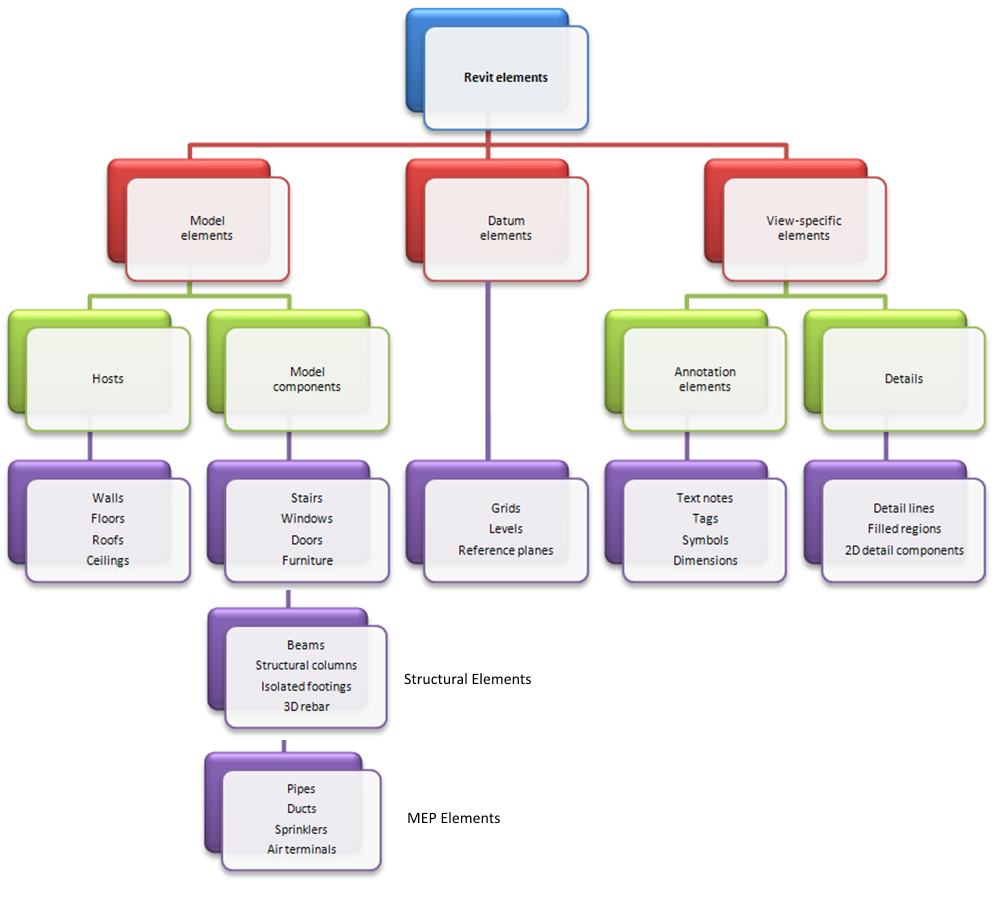
\includegraphics[width=\textwidth]{images/Revit-elements.png}
    \caption{Элементы информационной модели}
    \label{figure:RevitElements}
\end{figure}

\paragraph{Свойства элементов}

\lipsum[4]

\paragraph{Формат RVT}

\lipsum[4]

\comment{
    TODO:

    - Небольшое вступление о том, что речь идет только о Revit
    - Параметрическое моделирование (?)
        http://help.autodesk.com/view/RVT/2019/ENU/?guid=GUID-71F2C8EE-2A90-4076-A6C7-702082566DDF
    - Элементы информационной модели
        http://help.autodesk.com/view/RVT/2019/ENU/?guid=GUID-5BFA499A-5ACA-4069-852C-9B60C9DE6708
    - Свойства элементов
        http://help.autodesk.com/view/RVT/2019/ENU/?guid=GUID-1B5B5C2E-072F-4349-9C70-D88204F9145D
    - Формат rvt 
        Здесь еще написать, что для отображения будет производиться конвертация в fbx 

    Точно должна быть картинка из ревита с отелем!
        "Интерфейс Revit. Структура информационной модели."
    А еще вот эта картинка
        images\Revit-elements.png
        "Элементы информационной модели Revit"
}
